\kapitola{Literární rešerše}
\sekce {Problematika detekce duplicit v~datech}
Data jsou v~rámci různých ekosystémů ukládána v~různých formách. Liší se ve struktuře, pojmenování atributů a hlavně ve způsobu využívání unikátních identifikátorů datových entit. Ve chvíli, kdy se pokoušíme data z~takových různých zdrojů agregovat například do centrální databáze, vzniká problém. Tím je rozhodnout, které záznamy jsou unikátní a které se ve skutečnosti opakují a mají pouze jinou podobu kvůli odlišné struktuře dat nebo způsobu jejich získání.

Nekvalitní data jsou komplikací, která může vést k~zásadním chybám v~datové analýze a rozhodovacích procesech. Například ve zdravotnictví může mít existence duplicitních záznamů o~pacientech vážné důsledky – od nesprávně předepsaných léků až po chybné zdravotní statistiky.\cite{bess_problem_2024} V~oblasti e-commerce může duplicita zákaznických účtů znamenat špatně cílené marketingové kampaně nebo mylné vyhodnocení chování uživatelů.\cite{brown_8_2019} A~v~geoprostorových datech mohou duplicity vést k~nesprávné identifikaci lokací, chybným navigačním trasám nebo nesrovnalostem v~mapových podkladech.

Abychom mohli přesně popsat proces detekce duplicit, je nutné nejprve vyjasnit základní pojmy související s~datovými entitami a jejich reprezentací v~databázích.

\textbf{Entita} je obecný pojem označující reálný objekt nebo koncept, který má své vlastnosti a může být reprezentován v~datech. V~závislosti na kontextu může entitou být např. osoba, firma, geografický bod zájmu (POI) nebo administrativní oblast.

\textbf{Záznam} představuje konkrétní reprezentaci entity v~databázi. Jedna entita tak může být v~různých databázích reprezentován více různými záznamy, například s~mírně odlišnými údaji nebo formátem.

\textbf{Atribut} je konkrétní vlastnost nebo charakteristika entity, která ji popisuje a umožňuje její identifikaci v~databázích. Každý záznam obsahuje jeden nebo více atributů, přičemž některé atributy mohou být klíčové pro rozpoznání duplicit.
Atributy mohou být různých typů – například textové, číselné, kategorické nebo prostorové. V geolokačních datech bývají klíčovými atributy například souřadnice (zeměpisná šířka a délka), adresa, název místa nebo jeho typ (např. restaurace, park, obchodní centrum).

Duplicitní záznamy vznikají tehdy, když databáze obsahuje více reprezentací stejné entity, ať už kvůli chybám v~zápisu, rozdílnému formátu dat, nebo rozdílným zdrojům dat. V~literatuře se však termíny označující proces identifikace těchto duplicit ne vždy používají jednotně a často se jejich významy překrývají. Zatímco některé zdroje považují následující pojmy za synonyma, jiné mezi nimi rozlišují:

\begin{itemize}
  \item \textbf{Data matching} – proces porovnávání záznamů za účelem nalezení těch, které odpovídají stejné entitě, i když mají různé atributy nebo formáty. \cite{christen_data_2012}
  \item \textbf{Entity resolution} – proces slučování duplicitních záznamů do jednoho sjednoceného záznamu reprezentujícího danou entitu. \cite{quantexa_what_2024}
  \item \textbf{Record linkage} – propojení odpovídajících záznamů napříč různými databázemi, aniž by došlo ke sloučení do jedné reprezentace. \cite{stepanenko_what_2024}
\end{itemize}

To, že existují různé termíny pro podobné procesy, ukazuje, že problematika detekce duplicit vznikala nezávisle v~různých oborech, a proto je důležitější se soustředit na samotné postupy, než na přesné označení. \cite{christen_data_2012}

V~této práci bude hlavní pozornost věnována \textit{data matching}, tedy samotnému procesu hledání duplicitních záznamů v~datech, spíše než jejich následnému slučování (\textit{entity resolution}). Pro zajímavost, podle Google Trends je termín \textit{data matching} v~posledních pěti letech globálně vyhledávanější než ostatní zmiňované termíny. Viz obr. \ref{fig:google-trends-data-matching}.

\begin{figure}[htb]
  \centering
  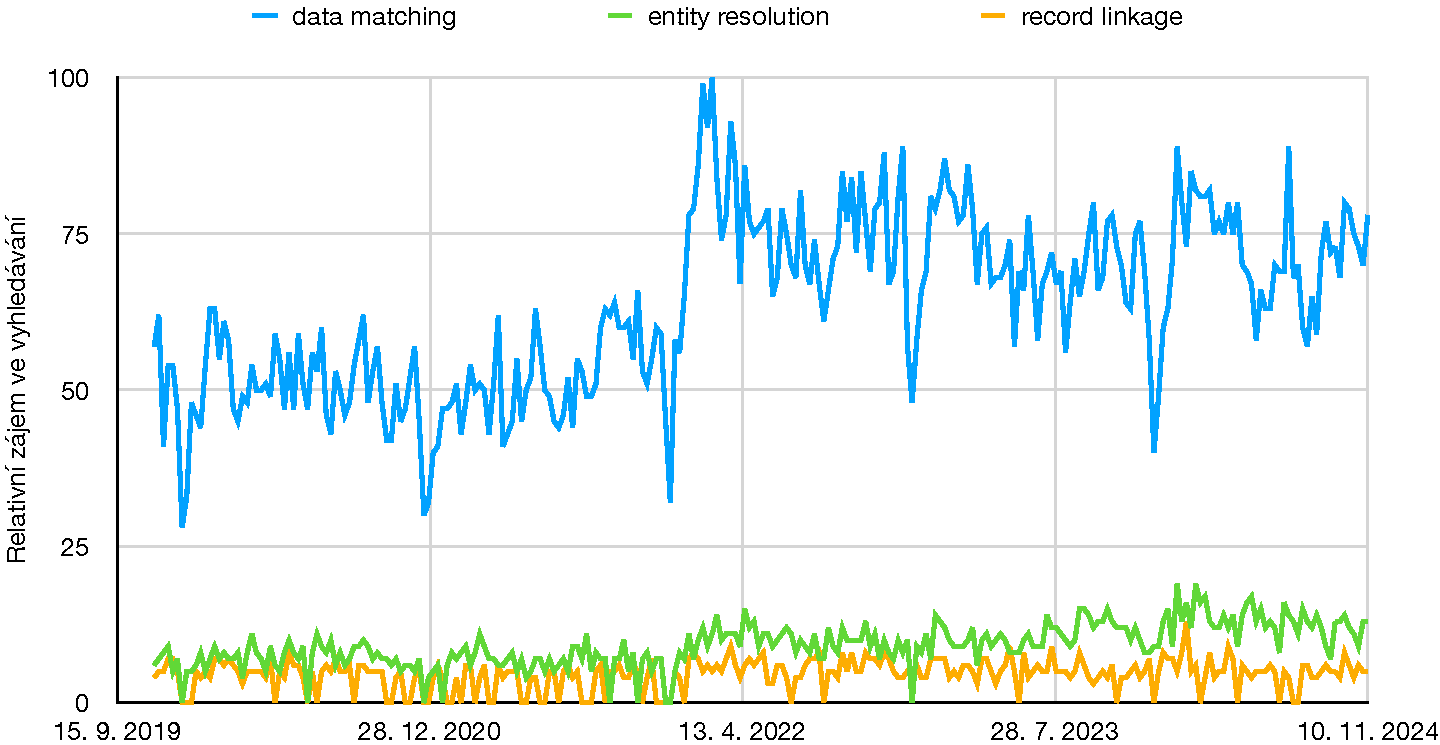
\includegraphics[scale=0.6]{images/google-trends.pdf}
  \caption{Zájem o~termíny "data matching", "entity resolution" a "record linkage".\newline
    \textit{Zdroj}: \cite{google_trends_google_2024}}
  \label{fig:google-trends-data-matching}
\end{figure}
\pagebreak

\sekce{Příčiny vzniku duplicit}
Zazněli zde již některé důvody vzniku duplicit v~datech, pojdmě se blíže podívat na nejčastější z~nich. Rozdělil jsem je zde na duplicity v~datech, které mohou vzniknout v~rámci jednoho datového zdroje, a duplicity vznikající spojením více datových zdrojů.

\podsekce{Duplicity v~samostatném zdroji}
Přestože by se na první pohled zdálo, že v~rámci jednoho datového zdroje šance na vznik duplicity minimiální, je zde i tak několik případů, které vedou ke vzniku duplicit. Tady jsou některé z~nich:

\begin{itemize}
  \item Lidský faktor – při zadávání dat člověkem ručně je velká pravděpodobnost zadání typografických chyb, různých nekonzistentních formátů a nebo přímo neplatných informací. Při zadávání dalších záznamů si pak daný člověk nemusí všimnout již existujícího záznamu vloženého dříve.
  \item Nedostatečné standardizace formátů – různé formuláře, dotazníky, nebo části/moduly jednoho systému mohou využívat různé formáty pro datumy, telefonní čísla, nebo rodná čísla a dalších typů dat. Pokud není správně ošetřen převod těchto dat do jednotného formátu před vložením záznamu, může opět docházet ke vzniku duplicit.
  \item Chybějící integritní omezení databáze – v~případě, že daná databáze nemá nastavená integritní omezení (např. na unikátní hodnoty v~rámci rodného čísla, IČO nebo třeba unikátnosti dvou a více atributů v~rámci jednoho záznamu), bude každý vložený záznam brán jako nový, doposud neexistující, záznam, přestože se může jednat o~identickou duplicitu.
\end{itemize}

\podsekce{Duplicity ve sloučeném zdroji}
Při pokusu o~spojení více zdrojů do jednoho vzniká několik výzev. V~rámci business inteligence se tento proces spojování různých datových zdrojů nazývá ETL\footnote{Extract, transform, load
}a v~rámci něj může docházet k~duplicitám v~několika případech:

\begin{itemize}
  \item Integrace různých systémů – v~případě systémů, které mají data o~entitách kvůli různým důvodům (např. inventární systém školy ukládá záznamy o~vybavení, online bazar má záznamy o~prodávaném vybavení), může vzniknout situace, kdy záznamy z~více systémů nelze spojit na základě společného unikátního klíče, protože má každý systém svůj unikátní pro danou entitu.
  \item Průběžné spojování dat – některé datasety jsou pravidelně aktualizované, aby co nejpřesněji odráželi realitu. Pokud však entita z~realného světa v~rámci aktuality změnila své atributy zásadně (např. pekárna se přestěhovala na jinou adresu a upravila své jméno), může vzniknout situace, kdy některý ze zdrojů bude mít stále staré údaje, a jiný nové, a tím pádem nepůjde tento rozdíl spojit s~původním záznamem a bude se milně jevit, že jde o~novou entitu.
  \item Rozdílné definice entit a identifikační metody – při integraci dat z~různých zdrojů se může stát, že jednotlivé systémy definují a identifikují stejné entity odlišně. Jeden systém může například využívat kombinaci jména, adresy a rodného čísla k~jednoznačné identifikaci osoby, zatímco jiný systém pracuje s~interním identifikačním číslem nebo používá jiné atributy (např. e-mailovou adresu). Tato nejednotnost vede k~tomu, že algoritmy pro slučování dat nemusí správně rozpoznat, že se jedná o~stejnou entitu, a následně dochází k~vytvoření duplicitních záznamů v~cílovém datovém skladu.
\end{itemize}

Toto zajisté nejsou všechny možné příčiny vzniku duplicit v~datech, měli by však nastínit, jak se jednotlivé příčiny mohou lišit, a proč se jedná o~problém, který nelze vyřešit univerzálním způsobem.

\sekce{Důsledky duplicitních dat}
Duplicitní data mohou mít na organizaci zásadní a mnohostranné dopady. Především se výrazně snižuje kvalita dat, informace se stávají nepřesnými, neúplnými a méně aktuálními. To ovlivňuje nejen tvorbu reportů, ale i analytické procesy, které jsou základem strategických rozhodnutí. Rozhodnutí vycházející z~chybně interpretovaných dat mohou vést k~nesprávným závěrům, což se může projevit například ve špatném plánování, neefektivním řízení zdrojů nebo dokonce v~riziku finančních ztrát.

Dalším významným důsledkem je snížení efektivity pracovníků. V~situaci, kdy je třeba trávit spoustu času identifikací a odstraňováním duplicit, se zaměstnanci odklánějí od jiných úkolů, které by mohly přinést přidanou hodnotu. Kromě rutinní práce, jako je kontrola a aktualizace záznamů, je také nutné dohledávat různé verze stejných dat, což výrazně komplikuje správu informací. Takový stav nejenže zvyšuje provozní náklady, ale také vede k~vyšší chybovosti a celkovému zhoršení kvality práce.

Nesmíme opomenout ani problémy spojené s~dodržováním regulatorních požadavků. Regulace často vyžadují přesné, konzistentní a bezpečné uchovávání dat. Duplicitní záznamy komplikují tvorbu přesných reportů, což může mít za následek sankce, pokuty nebo dokonce ztrátu důvěry ze strany regulačních orgánů, spolupracujících firem a zákazníků. Správa citlivých údajů, jako jsou osobní nebo finanční informace, se také stává náročnější, což představuje další riziko v~případě případných narušení bezpečnosti nebo při nutnosti vyhovět zákonným požadavkům na přístup a správu těchto dat.

Duplicitní data také negativně ovlivňují i zákaznický servis a správu IT infrastruktury. Když jsou informace o~zákaznících roztříštěny mezi několika duplicitními záznamy, je pro pracovníky obtížné získat ucelený přehled o~jejich historii, což vede ke zhoršení kvality poskytovaných služeb. Současně se tím zvyšuje náročnost správy datových logů, zálohovacích a archivních procesů.

Celkově lze říct, že neřešené duplicitní záznamy mají rozsáhlý negativní vliv na efektivitu, bezpečnost a spolehlivost informací v~organizaci. Firmy se snaží aktivně problém s~kvalitou dat řešit, a to ukazuje i průzkum "Big Data and AI Executive Survey 2024" od NewVantage Partners za rok 2023. Průzkumu se učasnilo více než 100 firem z~globálního Fortune 1000, a ukazuje, že pro většinu organizací (87,9\,\%) má investice do dat a analytiky vysokou prioritu. Ze stejného výzkumu však i vychází informace, že snaha o~zlepšení kvality dat byla úspěšná pouze u~37\,\% dotázaných firem.

\begin{figure}[htb]
  \centering
  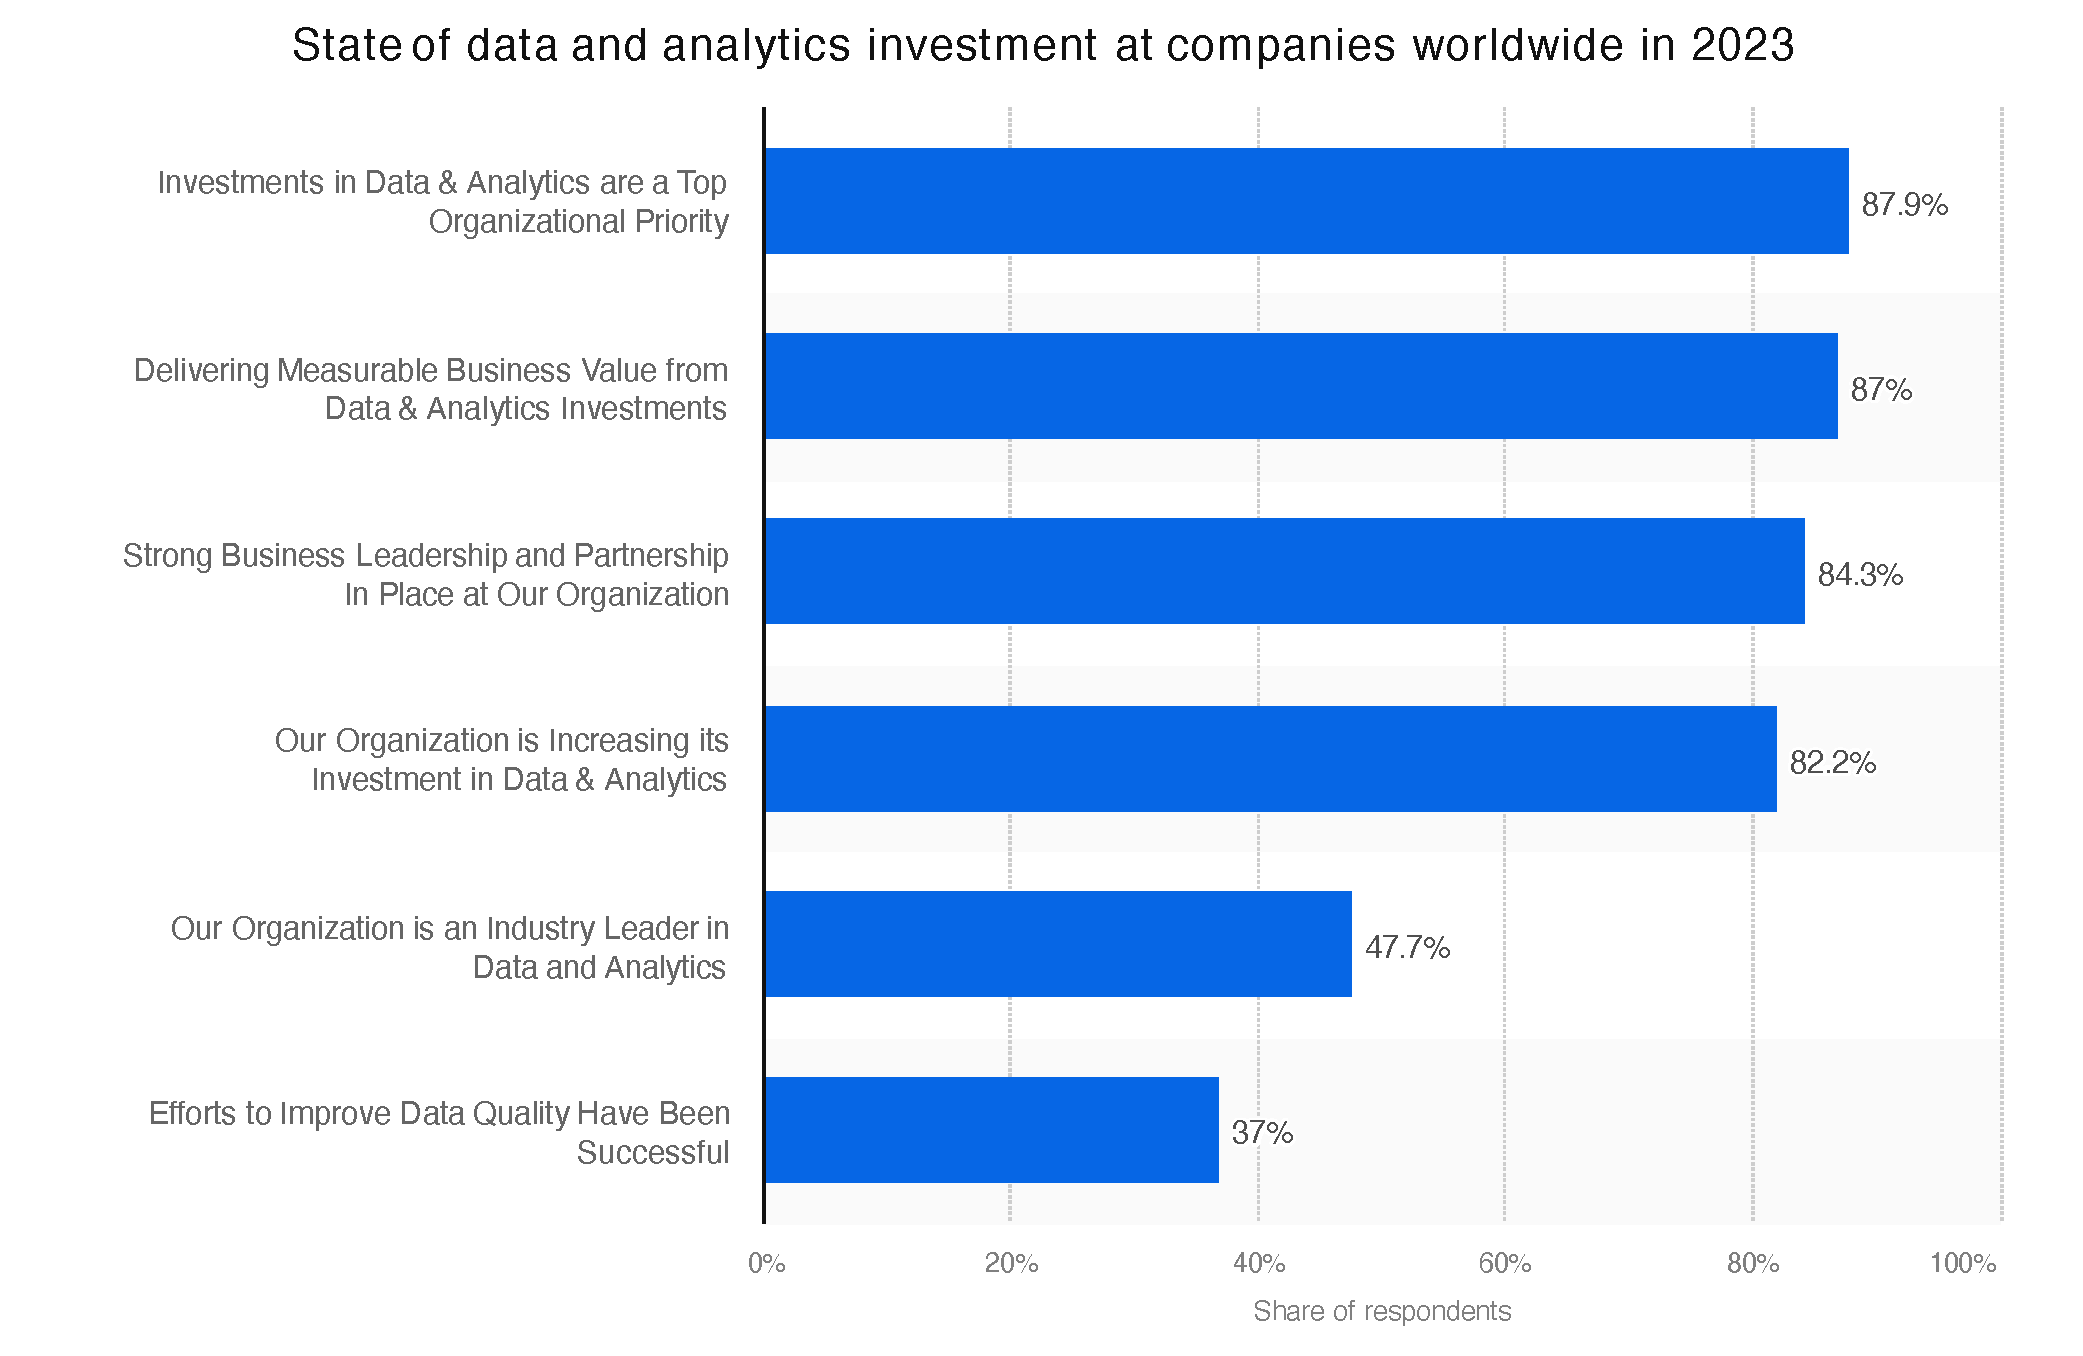
\includegraphics[width=\textwidth]{images/statista-global-state-of-data-and-analytics-investment-2023.pdf}
  \caption{Výsledky výzkumu o~investicích do dat a analytiky. \newline
    \textit{Zdroj}: \cite{newvantage_partners_global_2024}}
  \label{fig:google-trends-data-investing}
\end{figure}

\sekce {Obecné metody detekce duplicitních entit}
K řešení detekce duplicit je třeba využít kombinaci několika metod, které se vzájemně doplňují a umožňují zvýšit celkovou přesnost a robustnost systému. Následující podkapitola rozebírá jednotlivé skupiny přístupů, jejich fungování, výhody i nevýhody, a možnosti jejich vzájemného propojení.


\podsekce {Pravidla}
Jedná se o principielně jednoduchý přístup, který spočívá v tom, že se vytváří jednoznačná pravidla nebo sada pravidel, které podle daných kritérií určují duplicitní skupiny záznamů. Taková pravidla bývají navržena experty v dané oblasti, kteří vychází ze znalostí z oboru a charakteristik konkrétních dat.

Pravidla mají zpravidla jasně definované atributy, nebo skupinu atributů, které porovnávají a to buď striktně (hodnoty atributů musí být identické), kdy se jedná o tzv. exact matching, nebo volněji s použitím např. matematické logiky či prahových hodnot. Lze však kombinovat striktní a volnější porovnání v rámci složeného pravidla. To může slovně být popsáno třeba takto: \textit{„Dva záznamy jsou duplicity, pokud se shodují v atributu jméno a příjmení, mají shodné datum narození a současně rozdíl v jejich příjmech za poslední rok nepřesahuje 5 \%.“}.

K volnějšímu porovnání lze úvest i fonetické metody, které se používají primárně u textových údajů, které zní velice podobně, ale zapisují se různě. Jedná se například o Soundex, Metaphone a Double Metaphone, které z textového vstupu generují fonetické kódy, které lze následně porovnávat.

Výhodou takových pravidel je snadná implementace a jasná interpretace výsledků. Nicméně, vytvořená pravidla jsou málo flexibilní, jelikož jsou psaná vždy pro specificky typ dat, nebo pro konkrétní odvětví. V jednoduchých případech může takové řešení stačit, nicméně ve složitějších situacích může komplexnost takových pravidel růst a mohou být složitá na případná ladění a upravování. Pravidla však mohou sloužit jako dobrý první krok při zpracování dat, a na ně lze dále navázat další pokročilejší metody, které budou popsány v dalších sekcích.

\podsekce {Metody založené na podobnosti}

Metody založené na podobnosti identifikují duplicitní entity pomocí měření vzájemné podobnosti jednotlivých záznamů. Podobnost lze definovat jako míru blízkosti nebo podobnosti dvou entit na základě jejich atributů. Tyto metody jsou založeny na matematických metrikách, které kvantifikují míru podobnosti mezi dvojicemi atributů či celých záznamů.

Podobnost mezi dvěma entitami si lze představit jako číselnou hodnotu vyjadřující jejich vzájemnou shodu. Hodnota podobnosti bývá často definována v intervalu od 0 (žádná podobnost) do 1 (přesná shoda). K vyhodnocení podobnosti se používají různé metriky, které se zvolý na základě typu a charakteru porovnávaných atributů (text, čísla, časový údaj, atd.).

Mezi jednu z nejznámějších metrik patří \textbf{Levenshteinova vzdálenost}, která měří, kolik znaků je nutno přidat, odebrat, nebo změnit, aby se jeden řetězec stal identický s druhým. Výsledkem je číselná hodnota, která udává, kolik těchto operací se musí minimálně provést. Jde o metriku, která umožňuje snadno rozeznat například překlepy v krátkých řetězcích, ale v případě dlouhých řetězců mohou být vypočítané vzdálenosti vysoké.


Další známou metrikou je \textbf{Jaro-Winklerova podobnost}, která měří podobnost na základě počtu shodných znaků, jejich relativní vzdálenosti a počtu transpozic (špatného pořadí znaků). Krom toho také zohledňuje to, jestli porovnávané řetězce mají stejný začátek (prefix) a pokud ano, tak výrazně zvýší výslednou hodnostu podobnosti, která je v rozmezí 0 (zcela odlišné) a 1 (zcela shodné). Tato metrika je tedy lépe aplikovatelná na delší řetězce než zmíněná Levenshteinova vzdálenost, ale kvůli výpočetní náročnosti se často uvádí, že není ideální na porovnání dlouhých řetězců.

\textbf{Kosinová podobnost s TF-IDF} reprezentací je často používanou kombinací metod vhodnou především pro porovnávání delších textových dokumentů. TF-IDF\footnote{term frequency-inverse document frequency} transformuje texty do číselných vektorů, přičemž každému slovu v dokumentu přiřazuje váhu podle toho, jak často se vyskytuje v rámci konkrétního dokumentu (term frequency - TF) a jak vzácně nebo běžně se vyskytuje napříč celou kolekcí dokumentů (inverse document frequency - IDF). Slova, která se objevují často v mnoha dokumentech (např. běžné spojky či předložky), dostávají nižší váhu, zatímco specifická a méně častá slova obdrží váhu vyšší, čímž je zajištěno lepší zachycení významové relevance jednotlivých dokumentů. Kosinová podobnost následně měří podobnost dvou takto vzniklých vektorů dokumentů jako kosinus úhlu mezi nimi, přičemž výsledek se pohybuje mezi hodnotami 0 a 1, kde hodnota blízká 1 označuje velmi podobné dokumenty a hodnota blízká 0 označuje dokumenty s minimální nebo žádnou podobností. Velkou výhodou této metody je schopnost efektivně porovnávat obsah dokumentů bez zkreslení způsobeného různými délkami textů, a proto je tato technika široce využívána v oblasti vyhledávání informací, doporučovacích systémech, klasifikaci dokumentů a identifikaci duplicit, kde je potřeba přesněji zachytit tematickou nebo obsahovou podobnost textových záznamů.

\textbf{Jaccardova podobnost} představuje další často používanou metriku, která se zaměřuje na měření podobnosti množin atributů nebo znaků dvou entit. Tato metoda je založena na porovnání velikosti průniku (tedy počtu společných prvků) a velikosti sjednocení (tedy celkového počtu unikátních prvků v obou množinách). Výsledná hodnota Jaccardovy podobnosti se pohybuje mezi 0 (žádná shoda mezi množinami) a 1 (úplná shoda množin). Výpočet Jaccardovy podobnosti je jednoduchý, rychlý a dobře interpretovatelný, což ji dělá vhodnou pro různé aplikace, zejména tam, kde je potřeba porovnávat množiny diskrétních atributů, například množiny klíčových slov, tokenů, kategorií nebo uživatelů. Jednou z nevýhod této metriky však je to, že nezohledňuje frekvenci výskytu jednotlivých prvků, ale pouze jejich přítomnost nebo absenci. Jaccardova podobnost proto není ideální tam, kde je důležitá četnost prvků, například u analýzy textů, kde může být užitečnější kombinace s TF-IDF nebo jinými frekvenčními přístupy. Přesto se často využívá v systémech pro detekci duplicit, shlukování dokumentů a doporučovacích systémech.

Metody založené na podobnosti tedy představují efektivní přístupy k identifikaci duplicitních záznamů prostřednictvím různých matematických metrik, jejichž výběr závisí na typu a charakteru analyzovaných dat. Zatímco Levenshteinova vzdálenost a Jaro-Winklerova podobnost jsou ideální pro porovnávání krátkých nebo středně dlouhých textů, například při detekci překlepů či podobnosti názvů, Kosinová podobnost s TF-IDF reprezentací se osvědčuje především při práci s delšími dokumenty, kde je důležité zachytit obsahovou relevanci. Jaccardova podobnost zase vyniká svou jednoduchostí a rychlostí při porovnávání množin diskrétních atributů, jako jsou např. klíčová slova nebo tagy. V praxi se často osvědčuje vhodně kombinovat různé metriky nebo jejich varianty podle konkrétní situace, aby bylo dosaženo co nejpřesnějšího a nejspolehlivějšího výsledku při identifikaci duplicitních entit.

\podsekce {Pravděpodobnostní metody}
\todo{Definice a princip Fellegi-Sunterova modelu a jeho variant}
Pravděpodobnostní metody se zaměřují na modelování pravděpodobnosti, že dva záznamy odpovídají stejné entitě. Tyto metody využívají statistické modely a pravděpodobnostní teorie k~určení míry shody mezi záznamy. V~rámci těchto metod se často používá tzv. \textbf{Fellegi-Sunterův model}, který je jedním z nejznámějších a nejpoužívanějších přístupů k~identifikaci duplicitních záznamů.  Je založen na pravděpodobnostním modelu, který se snaží určit pravděpodobnost, že dva záznamy odpovídají stejné entitě, na základě jejich atributů. Tento model se skládá ze dvou hlavních komponentů: \textbf{pravděpodobnostní skóre} a \textbf{rozhodovací prah}. Pravděpodobnostní skóre je hodnota, která vyjadřuje míru shody mezi dvěma záznamy na základě jejich atributů. Rozhodovací prah je hodnota, která určuje, zda jsou dva záznamy považovány za duplicity nebo ne. Pokud je pravděpodobnostní skóre vyšší než rozhodovací prah, záznamy jsou považovány za duplicity. Jinými slovy, Fellegi-Sunterův model se snaží najít optimální rovnováhu mezi dvěma typy chyb: \textbf{falešně pozitivní} (kdy jsou dva záznamy považovány za duplicity, i když tomu tak není) a \textbf{falešně negativní} (kdy jsou dva záznamy považovány za různé, i když tomu tak je). Tento model se často používá v~kombinaci s~dalšími metodami, jako jsou metody založené na podobnosti nebo pravidla, aby se zvýšila přesnost a robustnost systému.
V~rámci pravděpodobnostních metod se také často používají různé varianty Fellegi-Sunterova modelu, které se zaměřují na specifické aspekty identifikace duplicitních záznamů. Například některé varianty se zaměřují na zohlednění různých typů atributů (např. textové, číselné, časové) nebo na zohlednění různých typů chyb (např. překlepy, různé formáty).
\todo{Možnosti aplikace bayesovských metod}
\todo{Výhody, nevýhody a limitace při použití}

\podsekce {Metody strojového učení}
\todo{Definice a typy (supervizované, semi-supervizované, nesupervizované)}
\todo{Typické algoritmy: rozhodovací stromy, Random Forest, Gradient Boosting}
\todo{Klíčové aspekty přípravy dat a výběr atributů}
\todo{Výhody, nevýhody}

\podsekce {Metody založené na hlubokém učení}
\todo{Princip neuronových sítí pro entity matching (např. embeddings, transformer modely)}
\todo{Scénáře nasazení a případové studie z literatury}
\todo{Omezení a nevýhody (black-box přístup, náročnost na data a výpočetní zdroje)}

\podsekce {Grafové metody}
\todo{Grafové přístupy k modelování entit}
\todo{Komunitní detekce, grafové neuronové sítě (GNN)}
\todo{Specifika aplikace, výhody, nevýhody}

\sekce {Specifické metody pro rozpoznání duplicit v~geolokačních datech}

\todo{Specifika geolokačních dat}
\todo{Prostorová přesnost a chyby měření}
\todo{Problematika výběru vhodných vzdálenostních metrik a projekcí}

\podsekce{Metody založené na vzdálenosti}
\todo{Popis a využití Haversinovy a Vincentyho vzdálenosti}
\todo{Aplikace vzdálenostních metod, výběr prahů}

\podsekce{Shlukovací (clusteringové) metody}
\todo{DBSCAN, HDBSCAN a OPTICS}
\todo{Typické scénáře použití v praxi}
\todo{Výhody a omezení metod}

\podsekce{Metody založené na prostorové mřížce (grid-based)}
\todo{Principy Geohashe a prostorových mřížek}
\todo{Scénáře využití a důsledky výběru velikosti mřížky}
\todo{Omezení metody a problémy s přesností}

\podsekce{Pravděpodobnostní a bayesovské metody}
\todo{Modelování prostorové nepřesnosti (GPS chyby)}
\todo{Příklady bayesovských přístupů ke geolokaci}
\todo{Výhody a limitace těchto metod}

\podsekce{Metody strojového učení a hlubokého učení v~geolokaci}
\todo{Stručně zmínit možnost aplikace ML přístupů, pokud to téma umožňuje}
\todo{Zvýraznit případové studie (pokud existují relevantní)}

\podsekce{Geokódování a porovnávání adres}
\todo{Standardizace adresních údajů}
\todo{Geokódovací nástroje a postupy}
